\documentclass[11pt,a4paper]{article}
\usepackage[margin=2cm]{geometry}\usepackage{tikz,xcolor,booktabs,tabularx}
\usetikzlibrary{arrows.meta,positioning,calc}
\definecolor{navy}{HTML}{223A5E}\definecolor{orange}{HTML}{D97735}\begin{document}\begin{center}{\color{navy}\Huge\bfseries PROJECT ROADMAP}\par\vspace{.2cm}{\large A quarterly calendar for visible dependencies}\end{center}
\section*{How to use this page} Put a decision, deliverable or review on the line when it has a real owner and date. Use the table below for detail; keep the timeline at decision level so it remains readable when the project changes.
\begin{center}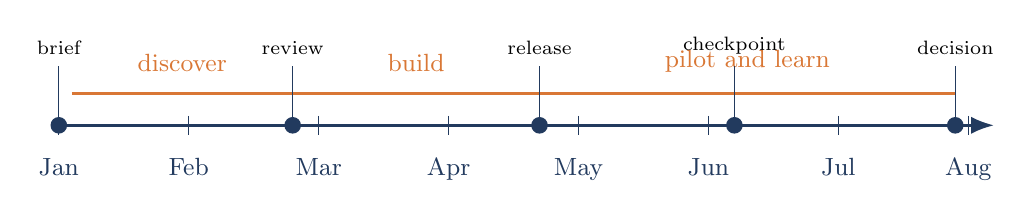
\begin{tikzpicture}[x=1.65cm,y=1cm,>=Latex]
\draw[very thick,navy,->] (0,0)--(7.2,0);\foreach \x/\m in {0/Jan,1/Feb,2/Mar,3/Apr,4/May,5/Jun,6/Jul,7/Aug}{\draw[navy] (\x,0.12)--(\x,-.12) node[below=5pt,font=\small]{\m};}
\draw[orange,very thick] (0.1,.4)--(1.8,.4) node[midway,above=4pt,font=\small]{discover};\draw[orange,very thick] (1.8,.4)--(3.7,.4) node[midway,above=4pt,font=\small]{build};\draw[orange,very thick] (3.7,.4)--(6.9,.4) node[midway,above=4pt,font=\small]{pilot and learn};
\foreach \x/\y/\t in {0/1/brief,1.8/1/review,3.7/1/release,5.2/1/checkpoint,6.9/1/decision}{\fill[navy] (\x,0) circle (3pt);\draw[navy] (\x,0)--(\x,.75);\node[above=.78cm,font=\scriptsize,align=center] at (\x,0){\t};}
\end{tikzpicture}\end{center}
\section*{Milestone register}\begin{tabularx}{\textwidth}{p{.16\textwidth}p{.2\textwidth}X p{.2\textwidth}}\toprule Date & Milestone & Exit evidence & Owner\\\midrule 15 Jan & Approved brief & Scope, budget and success measure signed off & Sponsor\\12 Feb & Discovery review & Five interviews summarised; top risks ranked & Product lead\\20 Mar & Pilot release & Test checklist complete; rollback path known & Delivery lead\\15 May & User checkpoint & Usage and feedback reviewed against baseline & Operations\\31 Jul & Go / change / stop & Decision memo with cost and evidence & Steering group\\\bottomrule\end{tabularx}
\section*{Dependencies and decisions}\begin{enumerate}\item Confirm access to the source data before building dashboards.\item Treat the March release as a pilot, not a production commitment.\item Record decision dates and decision-makers so later changes have an audit trail.\end{enumerate}\end{document}
